%%####################################################################
%    Copyright @ 2007 Andreas Frieß (Friess)
%    Permission is granted to copy, distribute and/or modify this document
%    under the terms of the GNU Free Documentation License, Version 1.2
%    or any later version published by the Free Software Foundation;
%    with no Invariant Sections, no Front-Cover Texts, and no Back-Cover Texts.
%    A copy of the license is included in the section entitled ``GNU
%    Free Documentation License''.
%%####################################################################
% Created: 28.08.2007
% @cvs($Date: 2007-09-05 19:46:18 +0000 (Wed, 05 Sep 2007) $)
% @cvs($Rev: 38 $)
% @cvs($Author: af0815 $)
% @cvs($URL: file:///svn/p/lazsnippets/code/trunk/dokumentation/LazSnippets/Kapitel/datenbanken/ProjektMySQLTestData.tex $)
%%####################################################################
\subsection{Projekt MySQLTestData}
\paragraph{Einleitung}
Es soll zeigen, wie man relativ einfach Testdaten in größerer Zahl in die Tabelle ST\_Person unserer Datenbank einfügt. Zugleich kann man es als Basis für Versuche mit SELECT Statements verwenden. In der Tabelle werden Lösch-, Einfüge- und Auswahloperationen durchgeführt.

\paragraph{Datenbank}
Es wird die Datenbank und Tabelle vom Beispiel \textbf{MySQLSimple} verwendet. Weitere Informationen können dort gefunden werden.

\paragraph{Benutzerschnittstelle}
Auf der Oberfläche befinden sich links drei Buttons. 
\parpic[sr][l]{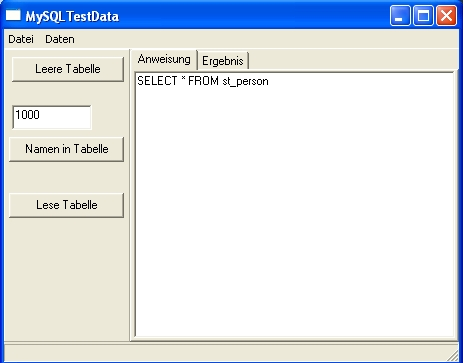
\includegraphics[width=0.25\textwidth]{Kapitel/datenbanken/pics/MySQLTestData01}} 
\caption{Projekt TestData GUI}
\label{fig:MySQLTestData01} 
Mit dem obersten Button wird die Tabelle komplett geleert, diese wird durch eine \emph{Delete} Anweisung im Quelltext durchgeführt. 
Der mittlere Button und das Eingabefeld darüber gehören zusammen und fügen neue Datensätze in der Tabelle ein. Die Anzahl der Datensätze wird durch den Wert im Eingabefeld vorgegeben.
Der unterste Button und das Tab-Sheet rechts daneben diesen zum Abfragen der Daten. Auf der ersten Seite des Tab-Sheets kann man das Abfrage Statement eingebn, die Anzeige erfolgt auf der zweiten Seite des Tab-Sheet.

Und jetzt die Funktionen mit den dahinterliegenden Code im Detail.
\subparagraph{Oberer Button}
Zuerst wird geprüft ob die Verbindung (Connection) zur Datenbank besteht, wenn nicht so wird die Verbindung hergestellt. Die Verbindungseinstelllungen wurden über den Objektinspektor schon beim Design getroffen, da es sich hier um Beispiele handelt.

\begin{verbatim}
if not MySQL50Connection1.Connected then
  MySQL50Connection1.Connected := true;
aSqlQuery := TSQLQuery.Create(self);
try
  aSqlQuery.SQL.Clear;
  aSqlQuery.DataBase := MySQL50Connection1;
  aSQLQuery.Transaction := SQLTransaction1;
  aSqlQuery.SQL.Add('DELETE FROM st_person;');
  aSqlQuery.ExecSQL;
finally
  aSqlQuery.free;
end;
\end{verbatim}

Anschliessend wird zur Laufzeit die TSQLQuery Komponente erzeugt. Wichtig ist, daß das Objekt erzeugt wird \verb|(aSqlQuery := TSQLQuery.Create(self);)|. Durch \emph{self} wird das Objekt dem Formular zugeordnet, so das das Formular beim Beenden auch das Objekt zerstören kann, falls es bis dahin noch nicht zerstört wurde.

Im nächsten Schritt wird ein eventuell vorhandenes gespeichertes SQL-Statement sicherheitshalber gelöscht. Weiters die Verbindung und die Transaktion zugewiesen. Dies geschieht genauso als würde man es über den Objektinspektor machen. Dann wird das neue SQL-Statement hinzugefügt. Da es ohne 'WHERE' EInschränkung verwendet wird, löscht es somit \textbf{alle} Daten aus der Tabelle. 

Zum Abschluß wird das verwendete SQL-Query Objekt wieder sauber entfernt. Damit dies auch geschieht wenn es einen Fehler gegeben hat, sind die Teile ab der Erstellung des Objektes durch ein try..finally Statement geklammert. Damit wird erreicht, das das Objekt auch nach einem Fehler richtig gelöscht wird.
\subparagraph{Mittlerer Button}
Beim betätigen des Buttons wird als erstes die Eingabe des Editfeldes überprüft und nur wenn der Wert in eine Zahl umgewndelt werden kann, wird fortgefahren.
\begin{verbatim}
try
  iAnzahl := StrToInt(edAnzahl.Text);
except
  showmessage('Nur Zahlen erlaubt');
  exit;
end;
\end{verbatim}

Mittels des Behfels \emph{randomize} wird der Zufallszahlengenerator initialisiert, dann die Verbindung zur Datenbank nötigenfalls hergestellt. Anschliessend eine TSQLQuery zur Laufzeit erzeugt und mit den nötigen Informationen versorgt.
\begin{verbatim}
randomize();
if not MySQL50Connection1.Connected then 
  MySQL50Connection1.Connected := true;
  
aSqlQuery := TSQLQuery.Create(self);
try
  aSqlQuery.SQL.Clear;
  aSqlQuery.DataBase := MySQL50Connection1;
  aSQLQuery.Transaction := SQLTransaction1;
\end{verbatim}
Weil wir später in einer Schleife Daten in die Datenbank einfügen, so erzeugen wir hier jetzt die nötigen Parameter. 

\textbf{HINWEIS:} Das Arbeiten mit Parametern ist wesentlich besser, als das Statement mittels Stringverwaltung zusammen zu setzen. Man vermeidet damit Probleme mit speziellen Zeichen, wie Hochkomma und der SQL-Server hat die Möglichkeit das Statement vor zu kompilieren und zu optimieren.

Anschliessend wird das SQL-Statement in die Query eingefügt. Mit den Doppelpunkt zeigt man, das es sich hier um einen Parameter handelt. 
\begin{verbatim}
  aSqlQuery.Params.CreateParam(ftInteger,'vname',ptInput);
  aSqlQuery.Params.CreateParam(ftInteger,'fname',ptInput);
  aSqlQuery.Params.CreateParam(ftInteger,'mname',ptInput);
  aSqlQuery.Params.CreateParam(ftInteger,'rname',ptInput);
  aSqlQuery.SQL.Add('INSERT st_person (cVName,cFName,cMName, cRName)');
  aSqlQuery.SQL.Add(' VALUES (:vname,:fname,:mname, :rname);');
\end{verbatim}
Hier beginnt die Schleife. ALs erstes werden dir Stringvariablen erzeugt, anschliessend die Strings den Parameteren übergeben.
\begin{verbatim}
  for i := 1 to iANzahl do
  begin
    iZufall := Random(MaxVorNamen-MinVorNamen) + MinVorNamen;
    cVName := VorNamen[iZufall];
    if cVName = '' then continue;

    iZufall := Random(MaxFamilienNamen-MinFamilienNamen) + 
                 MinFamilienNamen;
    cFName := FamilienNamen[iZufall];
    if cFName = '' then continue;

    cMName := leftStr(cVName,2)  +LeftStr(cFName,2);
    cRName := cVName + IntToStr(Random(10)) + cFName;

    aSqlQuery.Params.ParamByName('vname').AsString := cVName;
    aSqlQuery.Params.ParamByName('fname').AsString := cFName;
    aSqlQuery.Params.ParamByName('mname').AsString := cMName;
    aSqlQuery.Params.ParamByName('rname').AsString := cRName;
\end{verbatim}
Jetzt wird die Query mit den aktuellen Parametern durchgeführt. Der Befehl lautet \emph{ExecSQL}, dieser erwartet keine Ergebnismenge zurück. Das ist auch der Grund warum hier kein \emph{Open} oder \emph{Active=true} verwendet wurde, denn dieses erwarted das eine Ergebnismenge zurück geliefert wird. Anschliessend wird solange in der Schleife verblieben, bis alles abgearbeitet wurde. Wenn beim Ausführen ein Fehler auftritt, so wird in der Statuszeile eine Fehlermeldung angezeigt und mit dem nächsten durchlauf weitergemacht.
\begin{verbatim}
    try
      aSqlQuery.ExecSQL;
    except
      Statusbar1.SimpleText := 'Fehler in: ' + IntToStr(i);
      sleep(100);
    end;
  end;
finally
  aSqlQuery.free;
end;
\end{verbatim}

\subparagraph{Unterer Button}
Zum Unterschied vorher, ist diese Query zur Designzeit auf dem Formular hinterlegt worden. Damit entfällt das erzeugen zur Laufzeit. Das soll auch den Unterschied zwischen den beiden Methoden zeigen.

Es wird zuerst die Query inaktiv gemacht, falls sie offen war. Dann ganz einfach der Inhalt der Strings aus dem Meno in die Query übertragen und die Query wieder aktiv gemacht. Deshalb aktiv gemacht, da wir ja eine Ergebnismenge erwarten. Das hätten wir beim ausführen von \emph{ExecSQL} nicht.
\begin{verbatim}
  if SQLQuery1.Active then SQLQuery1.Active := false;
  SQLQuery1.SQL.Clear;
  SQLQuery1.SQL.Assign(Memo1.Lines);
  try
    SQLQuery1.Active := true;
  except
    showmessage('Anweisungen nicht gültig');
  end;
\end{verbatim}
Dann kann man im Datengitter die Ergebnisse betrachten.


\paragraph{SVN}
Den Quelltext des Beispiel kann man sich auch mit folgenden Kommando aus dem SVN ind das aktuelle Verzeichnis holen.
\begin{verbatim}
svn co https://lazsnippets.svn.sourceforge.net/svnroot/lazsnippets/\
  trunk/datenbank/MySQL/MySQLTestData .
\end{verbatim}
Die Zeile ist in einem zu schreiben und wurde nur aus Formatierungsgründen hier beim Rückstrich (Backslash) umgebrochen. Der Punkt am Ende der Zeile ist notwendig, da es das Kennzeichen für das aktuelle Verzeichnis ist. Weiter ist auf die Schreibweise zu achten, das hier die Server zwischen Großbuchstaben und Kleinbuchstaben unterscheiden.

\paragraph{Version}
\begin{table}[htbp]
%	\centering
		\begin{tabular}[ht]{|l|l|}
      \hline
      Betriebssystem & getestet \\
      \hline
%      Linux Unbuntu & nein \\
      Linux Suse & nein \\
%      Linux Debian & nein \\
%      Win95 + WinME & nein \\
%      Win2k & nein \\
      WinXP & ja \\
%      WinVista & nein \\
      \hline
		\end{tabular}
\end{table}
\caption{Versionsübersicht}
\label{tab:MySQLTestDataVersion01} 

\verb|Version: $LastChangedRevision: 38 $ |\footnote{ Autor: Andreas Frieß\\Lizenz: GFDL}